\documentclass{beamer}
\setbeamertemplate{caption}[numbered]
\usepackage{multirow}
\usepackage{fancyhdr}
\usepackage{graphicx}
\graphicspath{{../images/}}
\usepackage{multimedia}
\usepackage{color}
\usepackage{caption}
\usepackage{wrapfig}
\usetheme{Berlin}  %{Berlin}{Hannover}{Singapore}{CambridgeUS}

\title{Automatic Image Colorization using Generative Adversarial Networks}
\subtitle{\textbf{Team}: Yet Another Layer - YAL}


\author{Cameron Fabbri, Md Jahidul Islam}

\begin{footnotesize}

\end{footnotesize}


\begin{document}
\date{}
%%%%%%%%%%%%%%%%%%%%%%%%%%%%%%%%%
\begin{frame}
\thispagestyle{empty}
\titlepage
\end{frame}
%%%%%%%%%%%%%%%%%%%%%%%%%%%%%%%%%

\section*{Preliminaries}
%%%%%%%%%%%%%%%%%
\begin{frame}
\frametitle{\textbf{Image Colorization}}

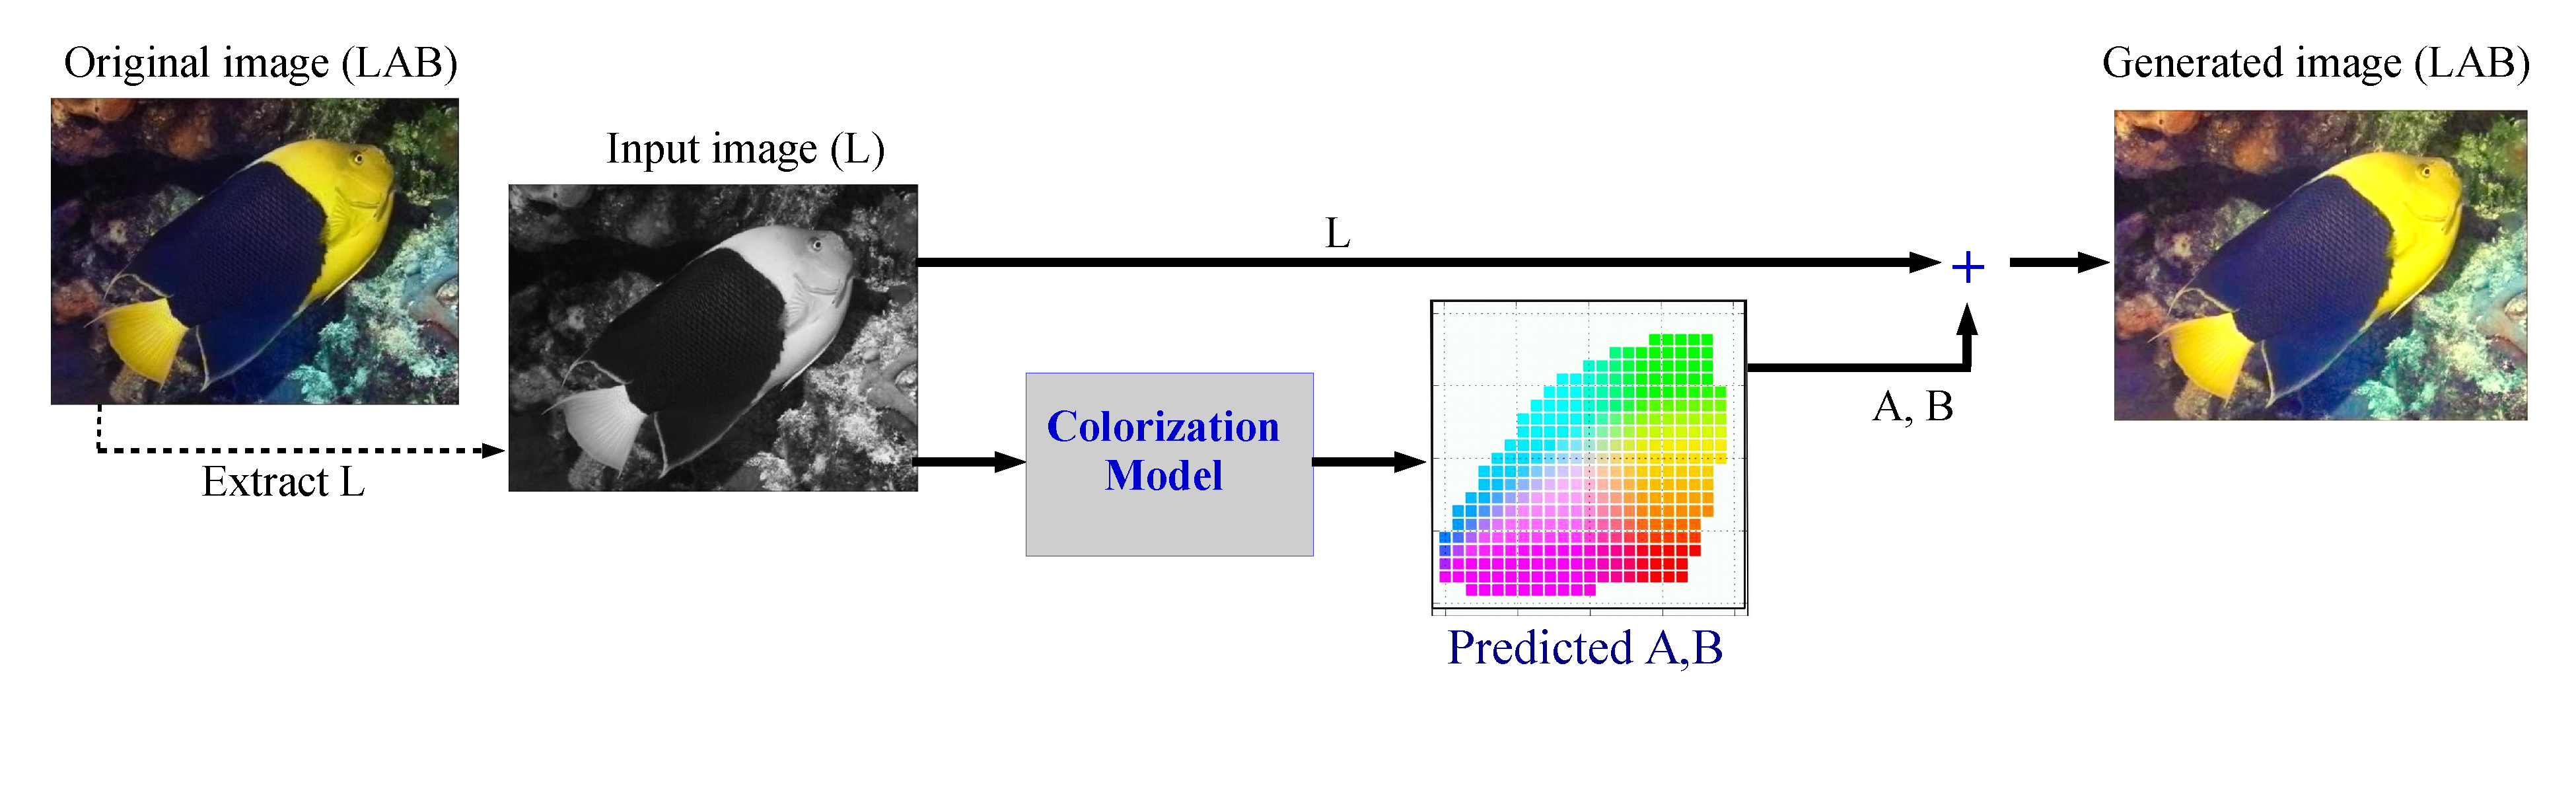
\includegraphics[width=\linewidth]{6.pdf}



\end{frame}

%%%%%%%%%%%%%%%%%% Background
\begin{frame}
\frametitle{\textbf{Background}}
\begin{itemize}
  \item Algorithmic choices:
	\begin{enumerate}[$-$]
	\item  \textbf{Image-to-image translation} 
	\item Classification
	\end{enumerate}
	
	\item Colorspace choices:
  
	\begin{enumerate}[$-$]
	\item  \textbf{LAB}, RGB
	\end{enumerate}
	
	\item Approaches
  
	\begin{enumerate}[$-$]
	\item Classical
	\item Deep learning based
	\begin{enumerate}[$-$]
	  \item Generative models
	  \item \textbf{Adversarial model}
	\end{enumerate}	 
	\end{enumerate}
	
\end{itemize}
\end{frame}
%%%%%%%%%%%%%%%%%%%%%%%

%%%%%%%%%%%%%%%%%%%%%%%
\section*{Classical Models}
\begin{frame}
\frametitle{\textbf{Classical Approaches}}
\framesubtitle{\textbf{Colorization using User-specified Prior [4]}}
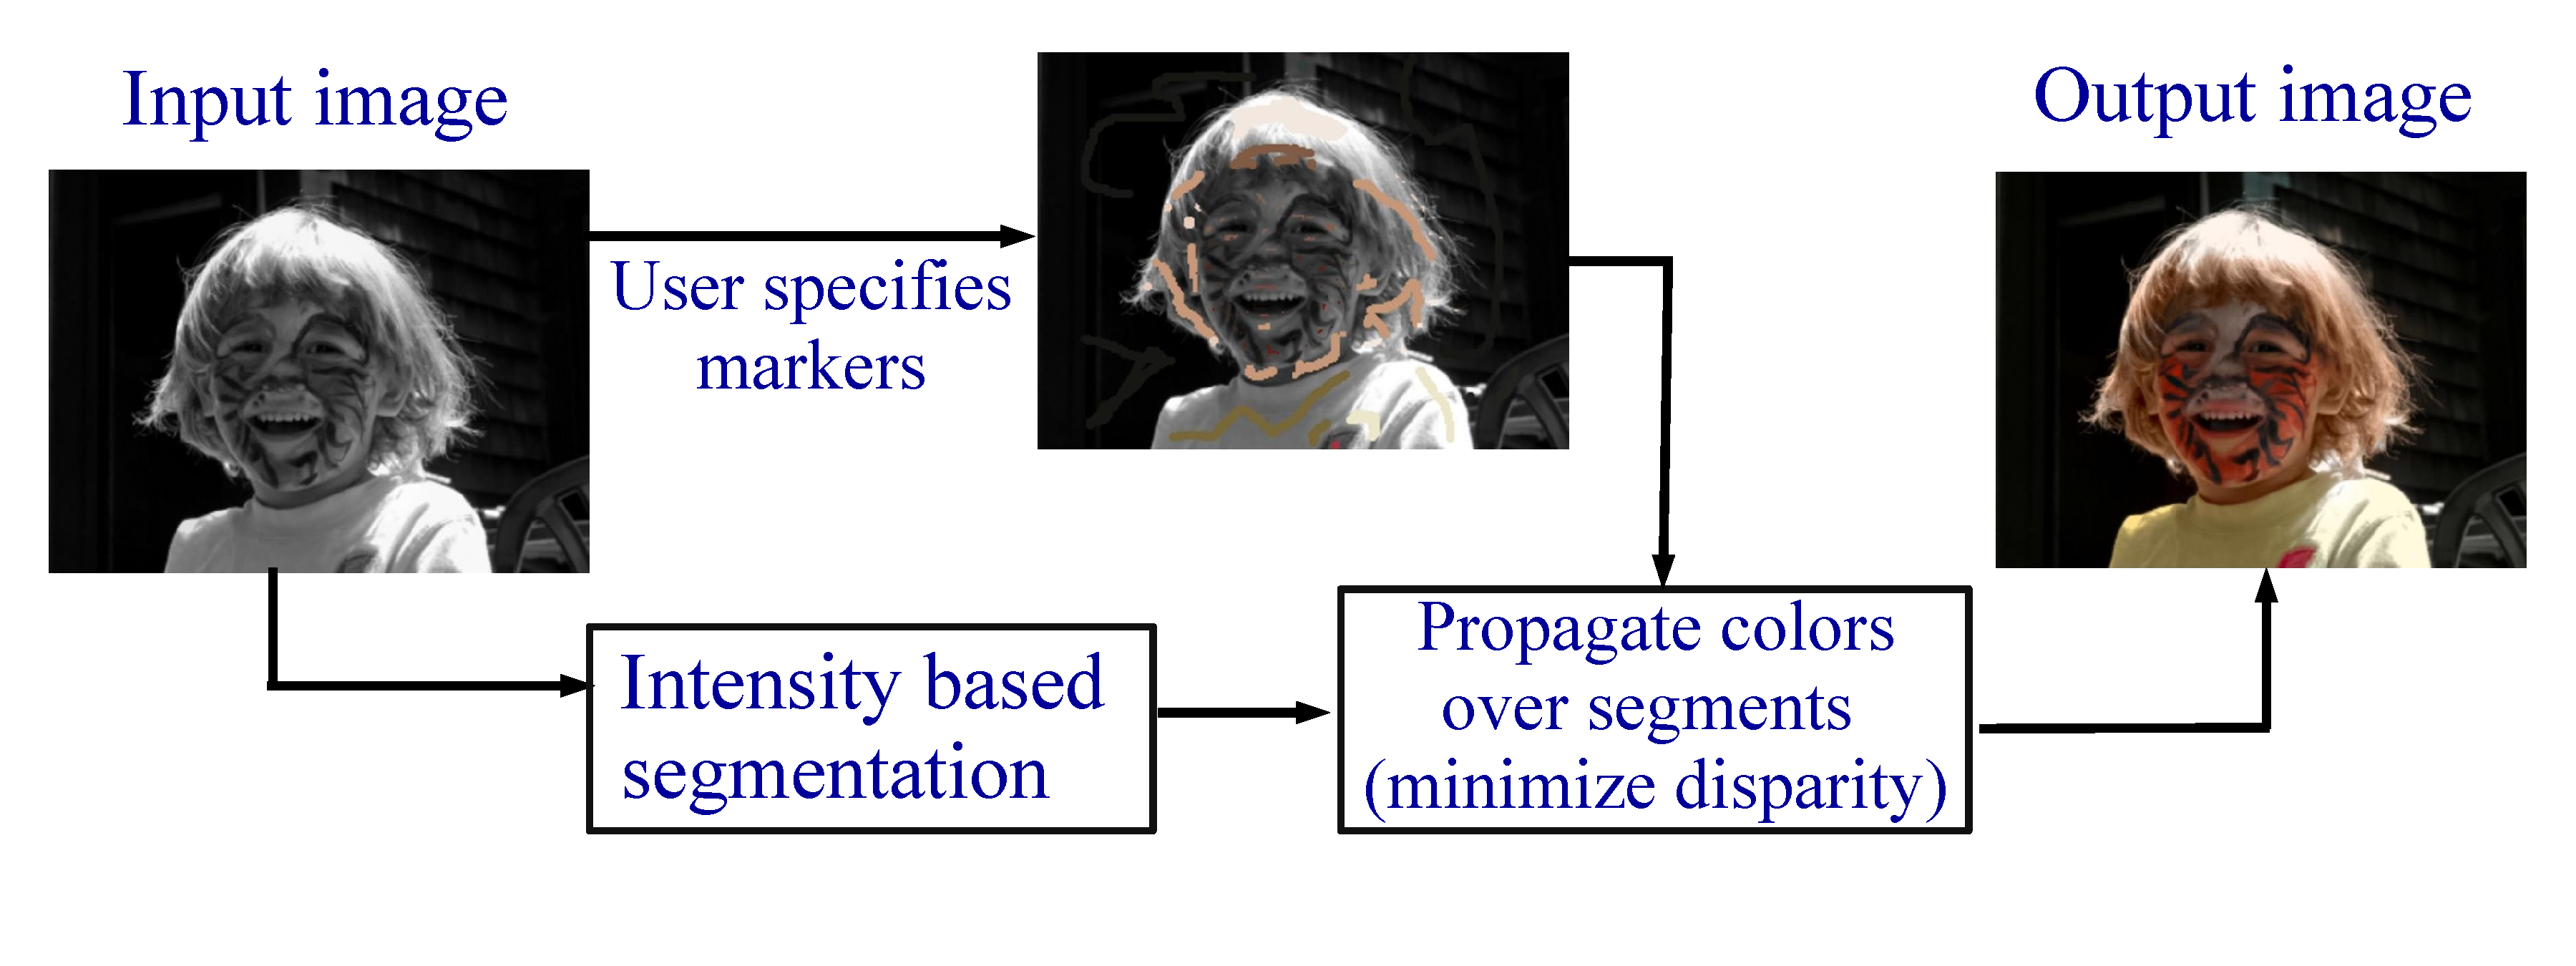
\includegraphics[width=\linewidth]{5.pdf}

\vspace{-3mm}
\begin{table}

\centering
\begin{tabular}{llll}
{\color{blue} \textbf{Pros}} & & & {\color{red} \textbf{Cons}} \\
Fast & & & Not automatic \\
Reliable & & & Not scalable

\end{tabular}
\end{table}

\end{frame}

\begin{frame}
\frametitle{\textbf{Classical Approaches}}
\framesubtitle{\textbf{Colorization using Multi-modal Prediction [5]}}
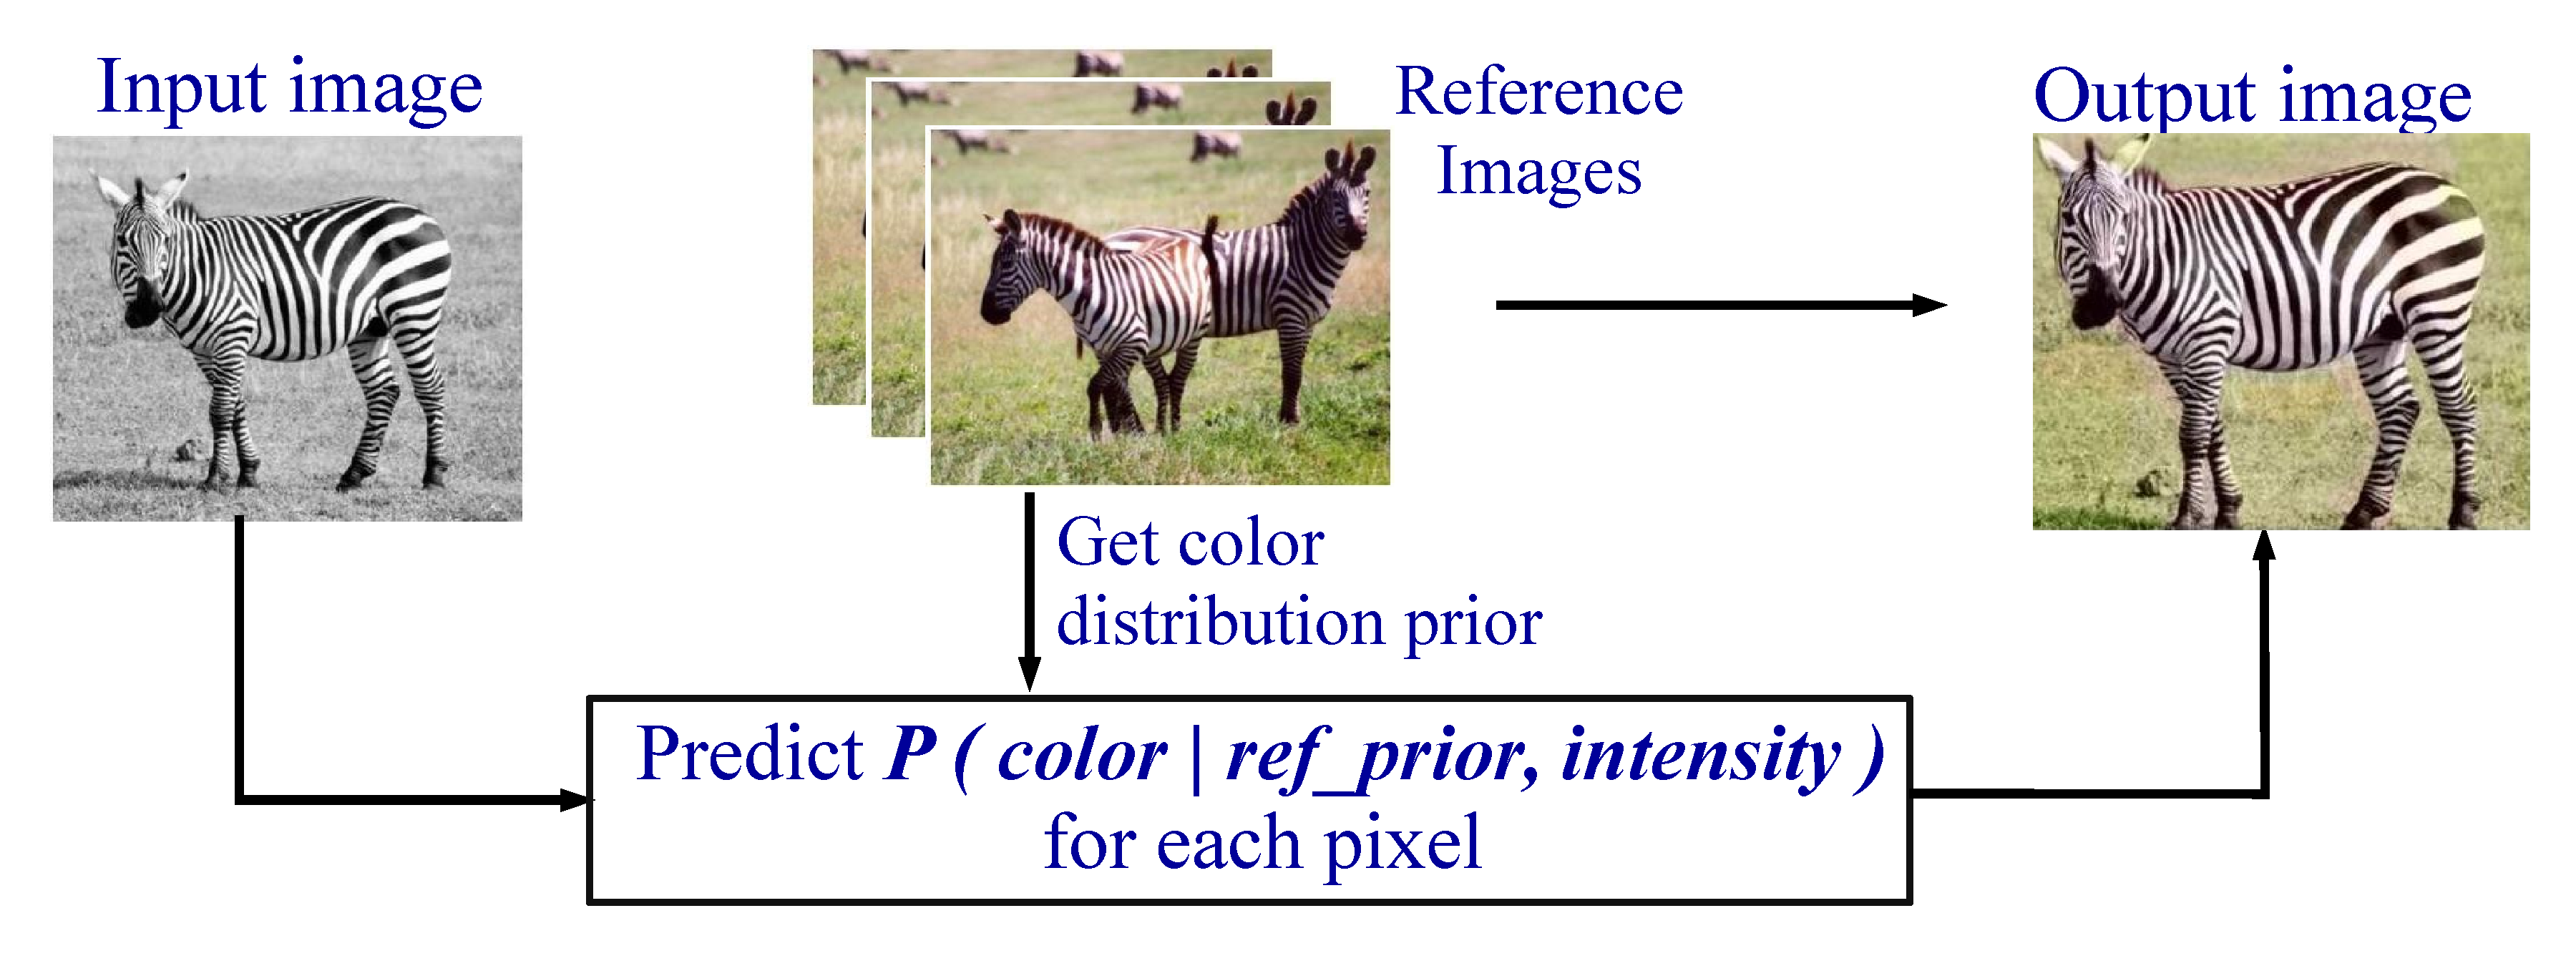
\includegraphics[width=\linewidth]{4.pdf}

\vspace{-5mm}
\begin{table}
\centering
\begin{tabular}{llll}
{\color{blue} \textbf{Pros}} & & & {\color{red} \textbf{Cons}} \\
Automatic & & & Depends heavily on reference prior  \\
Handles multimodality & & & Not practical

\end{tabular}
\end{table}

\end{frame}


\section*{DL: Generative Models}

\begin{frame}
\frametitle{\textbf{Generative Approach}}
\framesubtitle{\textbf{Colorful Image Colorization model [1]}}
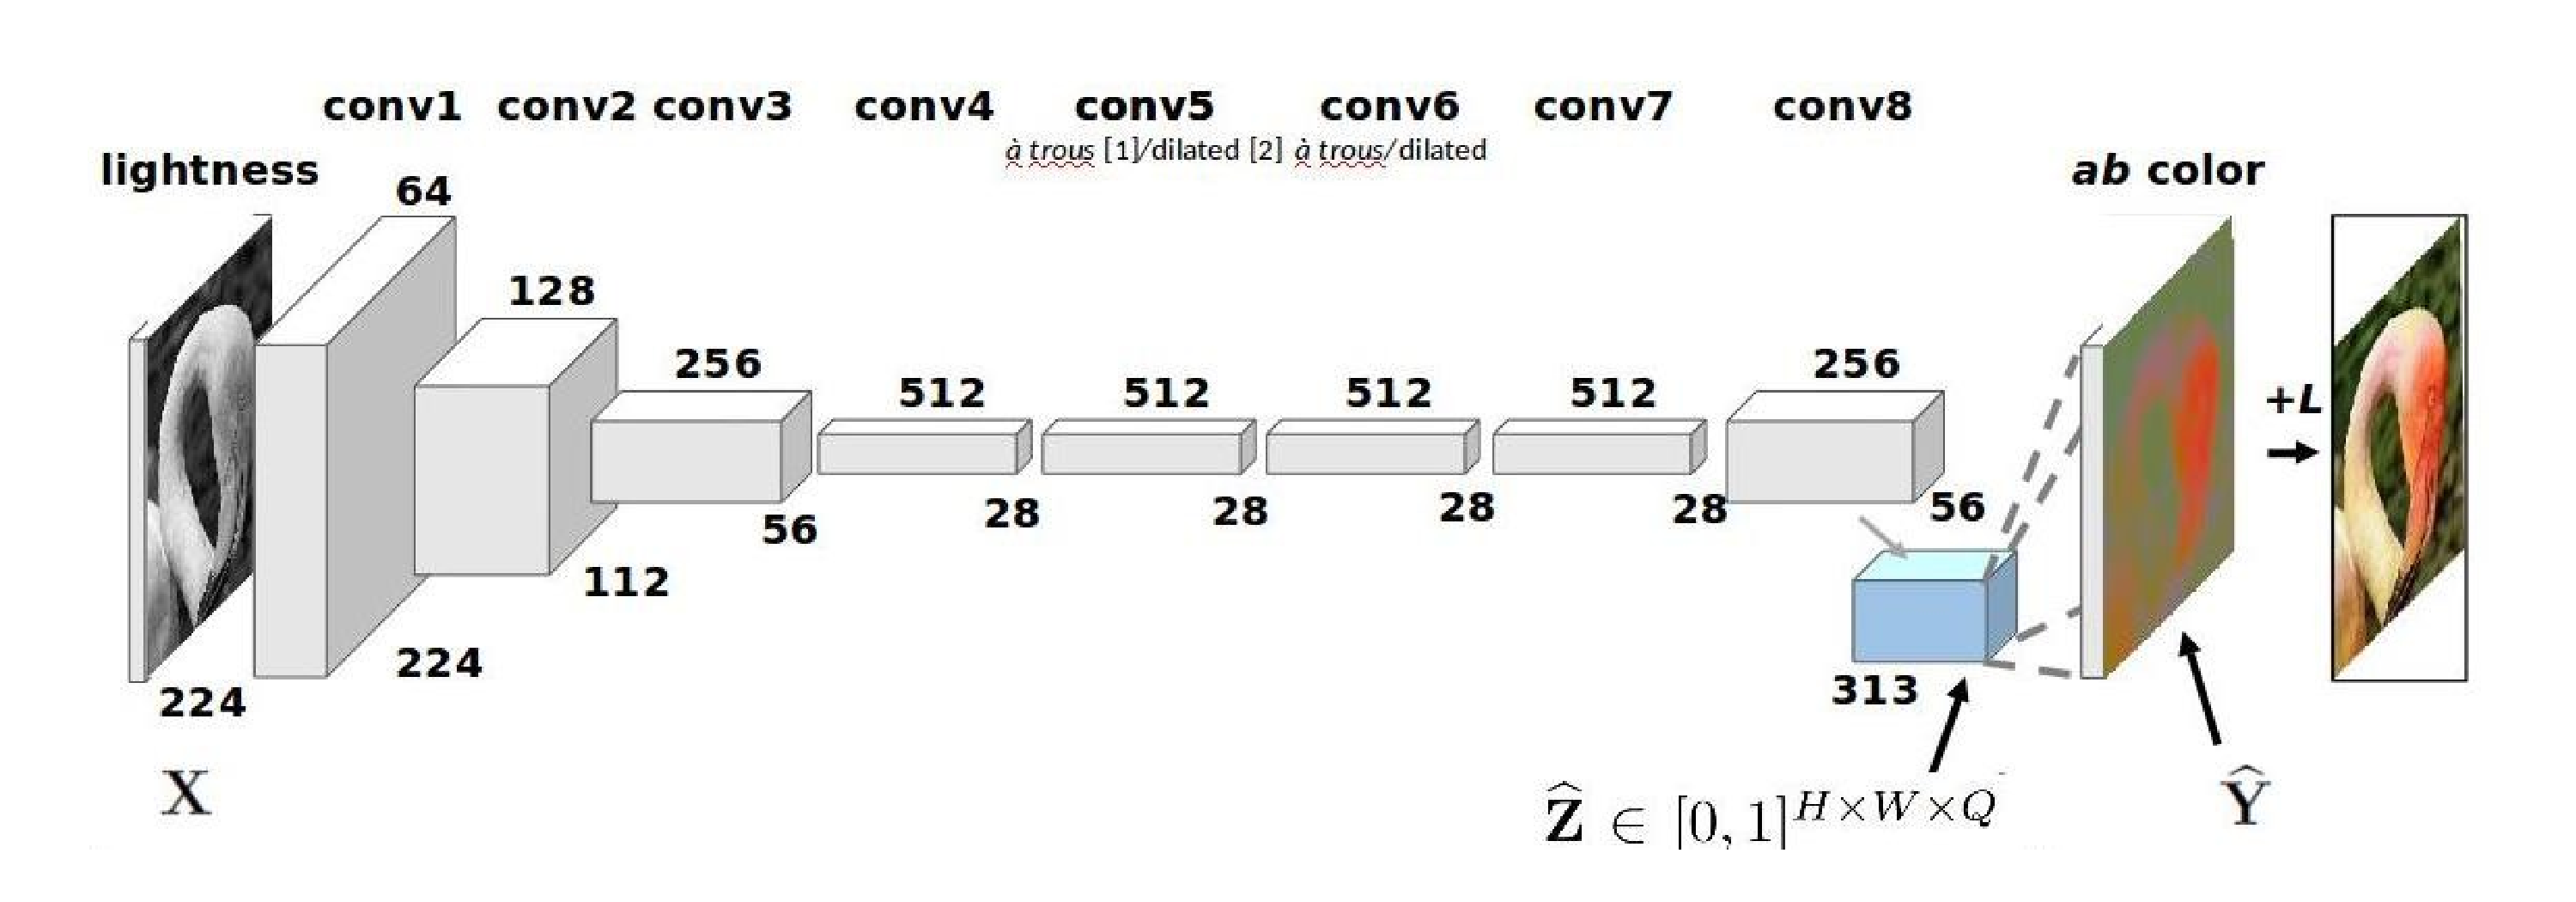
\includegraphics[width=\linewidth]{7.pdf}


\begin{table}
\footnotesize
\centering
\begin{tabular}{|l|l|l|}
\hline 
\textbf{Model Changes} & {\textbf{Original model}}  & {\color{blue} \textbf{Adopted model}} \\
\hline \hline
Output & Classification  Probabilities & {\color{blue} Image}  \\ \hline
Trained on & ImageNet & {\color{blue} CelebA, Places2 }\\ \hline
Implementation & Caffe & {\color{blue}Tensor-flow} \\ \hline

\end{tabular}
\end{table}

\end{frame}

\begin{frame}
\frametitle{\textbf{Results}}
\framesubtitle{\textbf{Colorful Image Colorization model as generator only}}
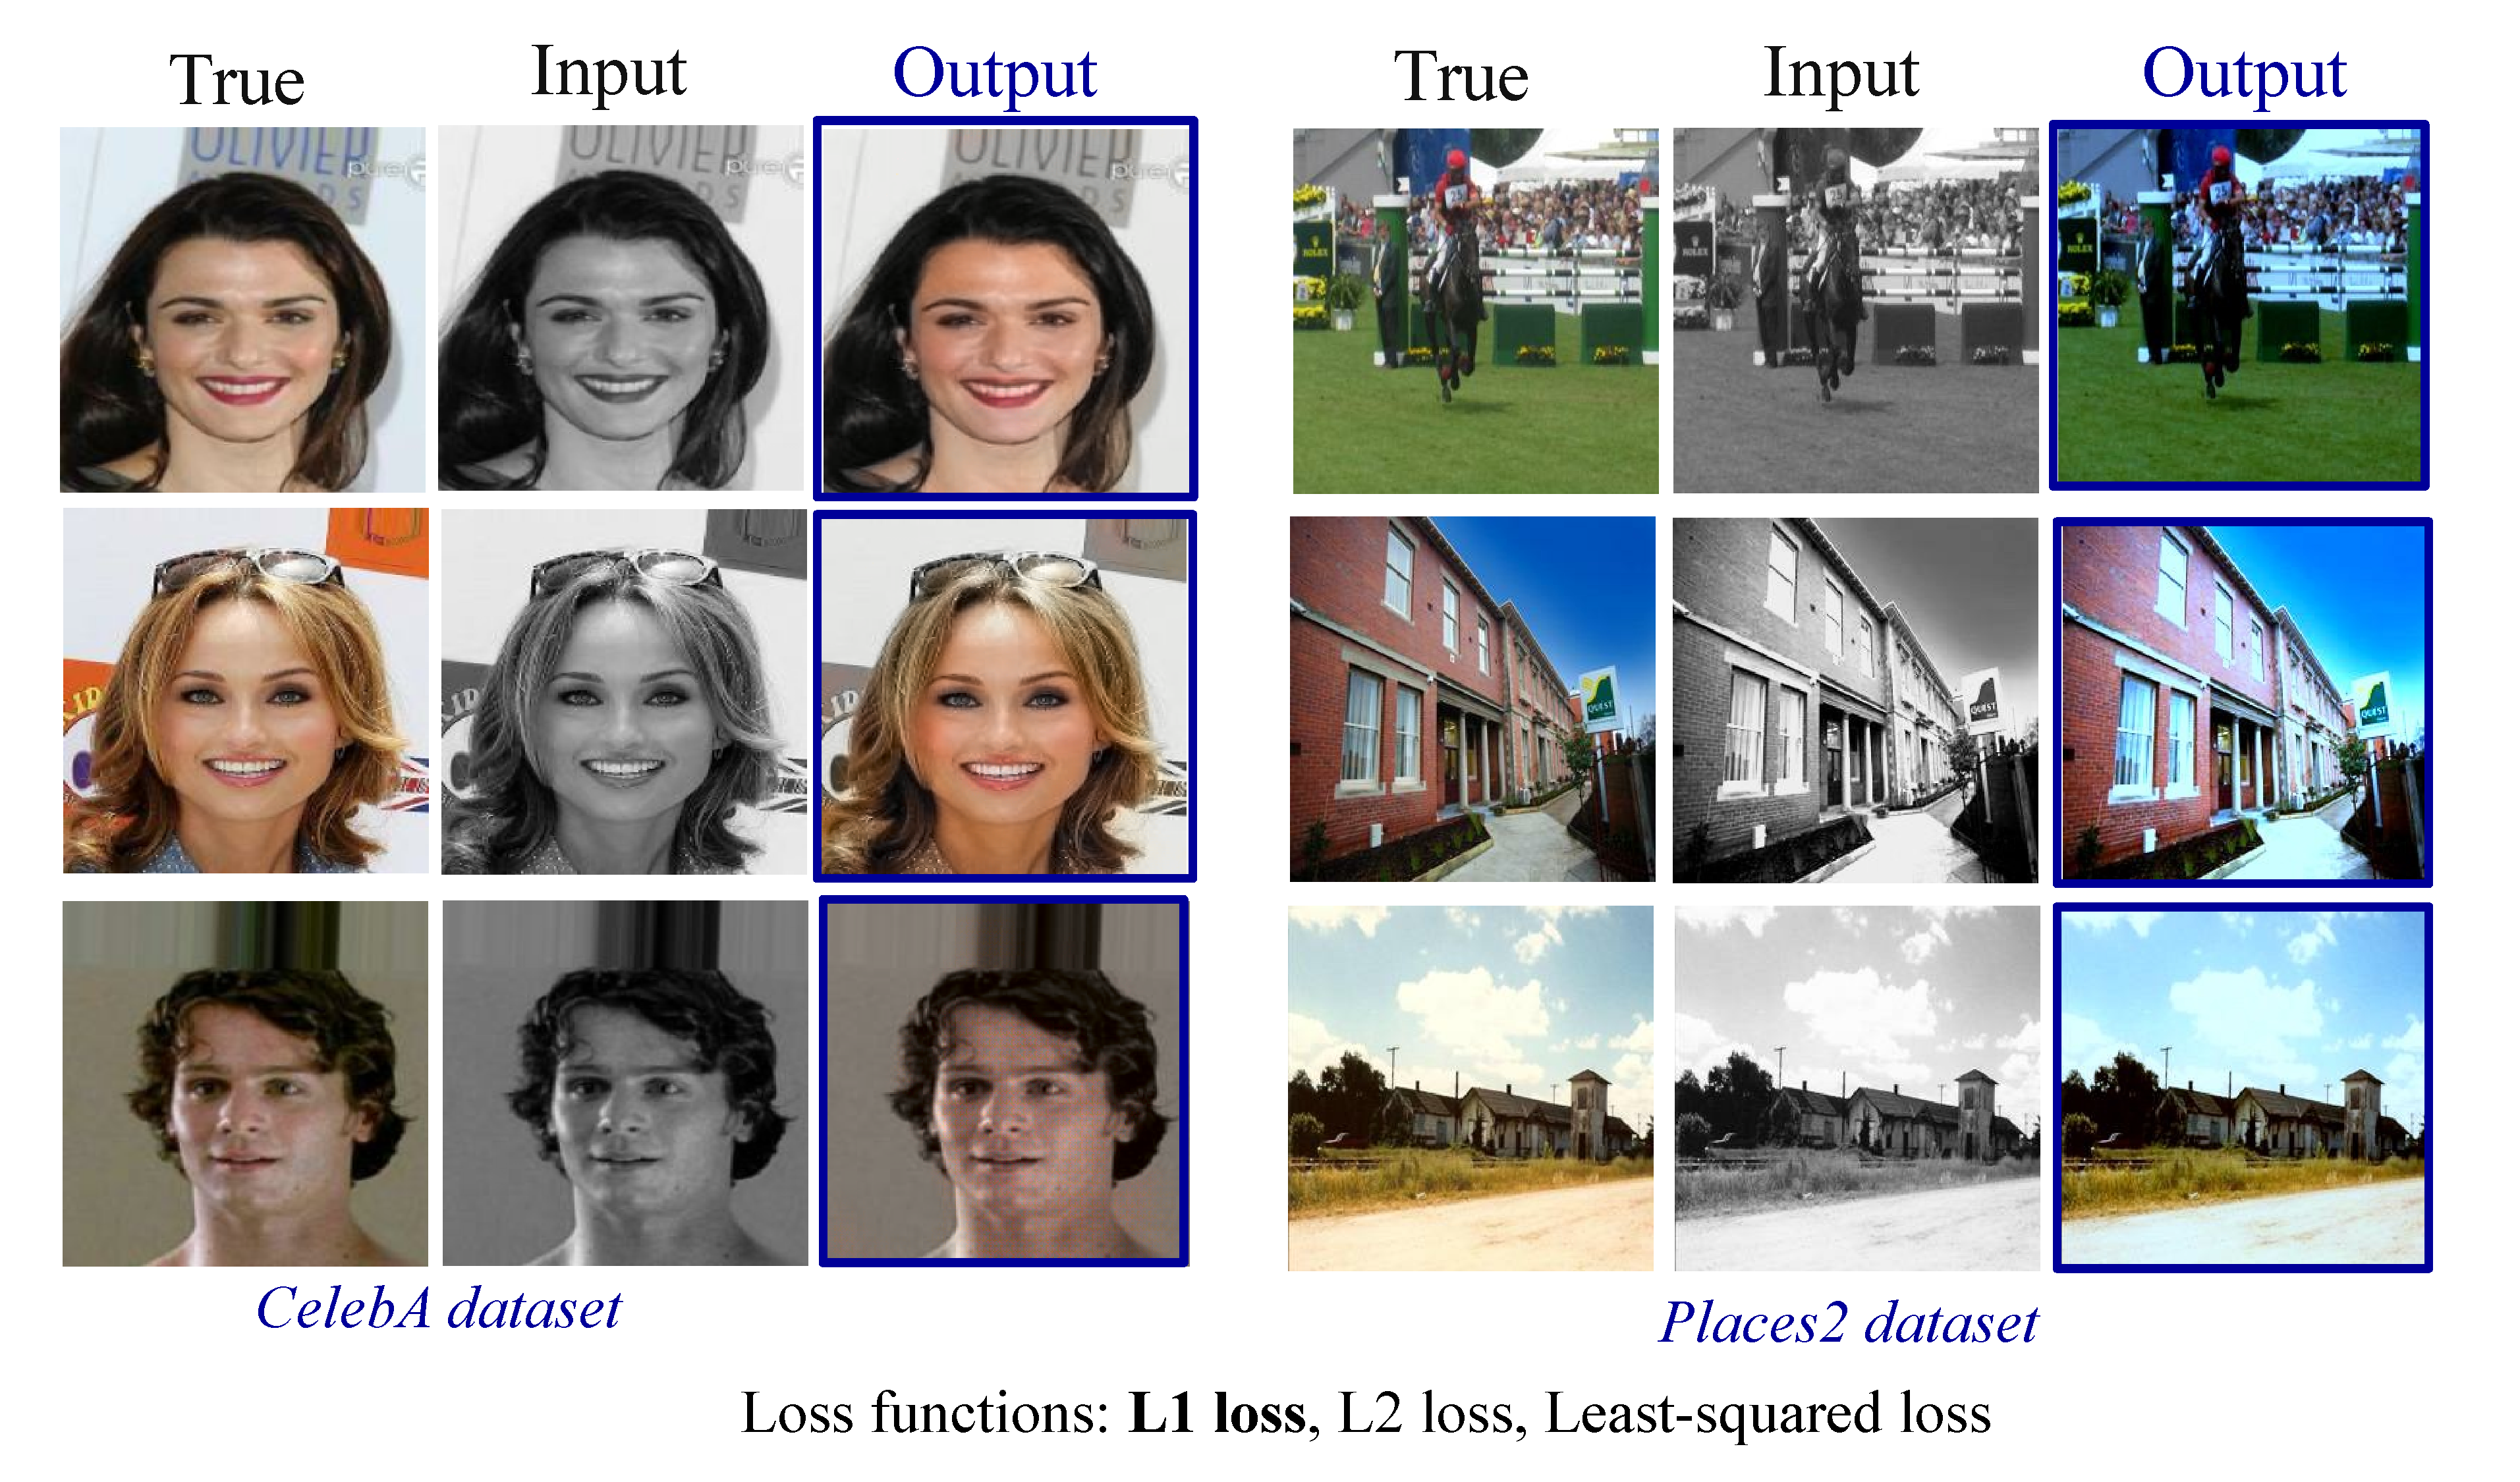
\includegraphics[width=\linewidth]{81.pdf}
\end{frame}

%%%%%%%%%%%%%%%%%%%%%%%%% GANs
\section*{DL: Adversarial Models}
\begin{frame}
\frametitle{\textbf{Results}}
\framesubtitle{\textbf{Colorful Image Colorization model as generator in a GAN}}
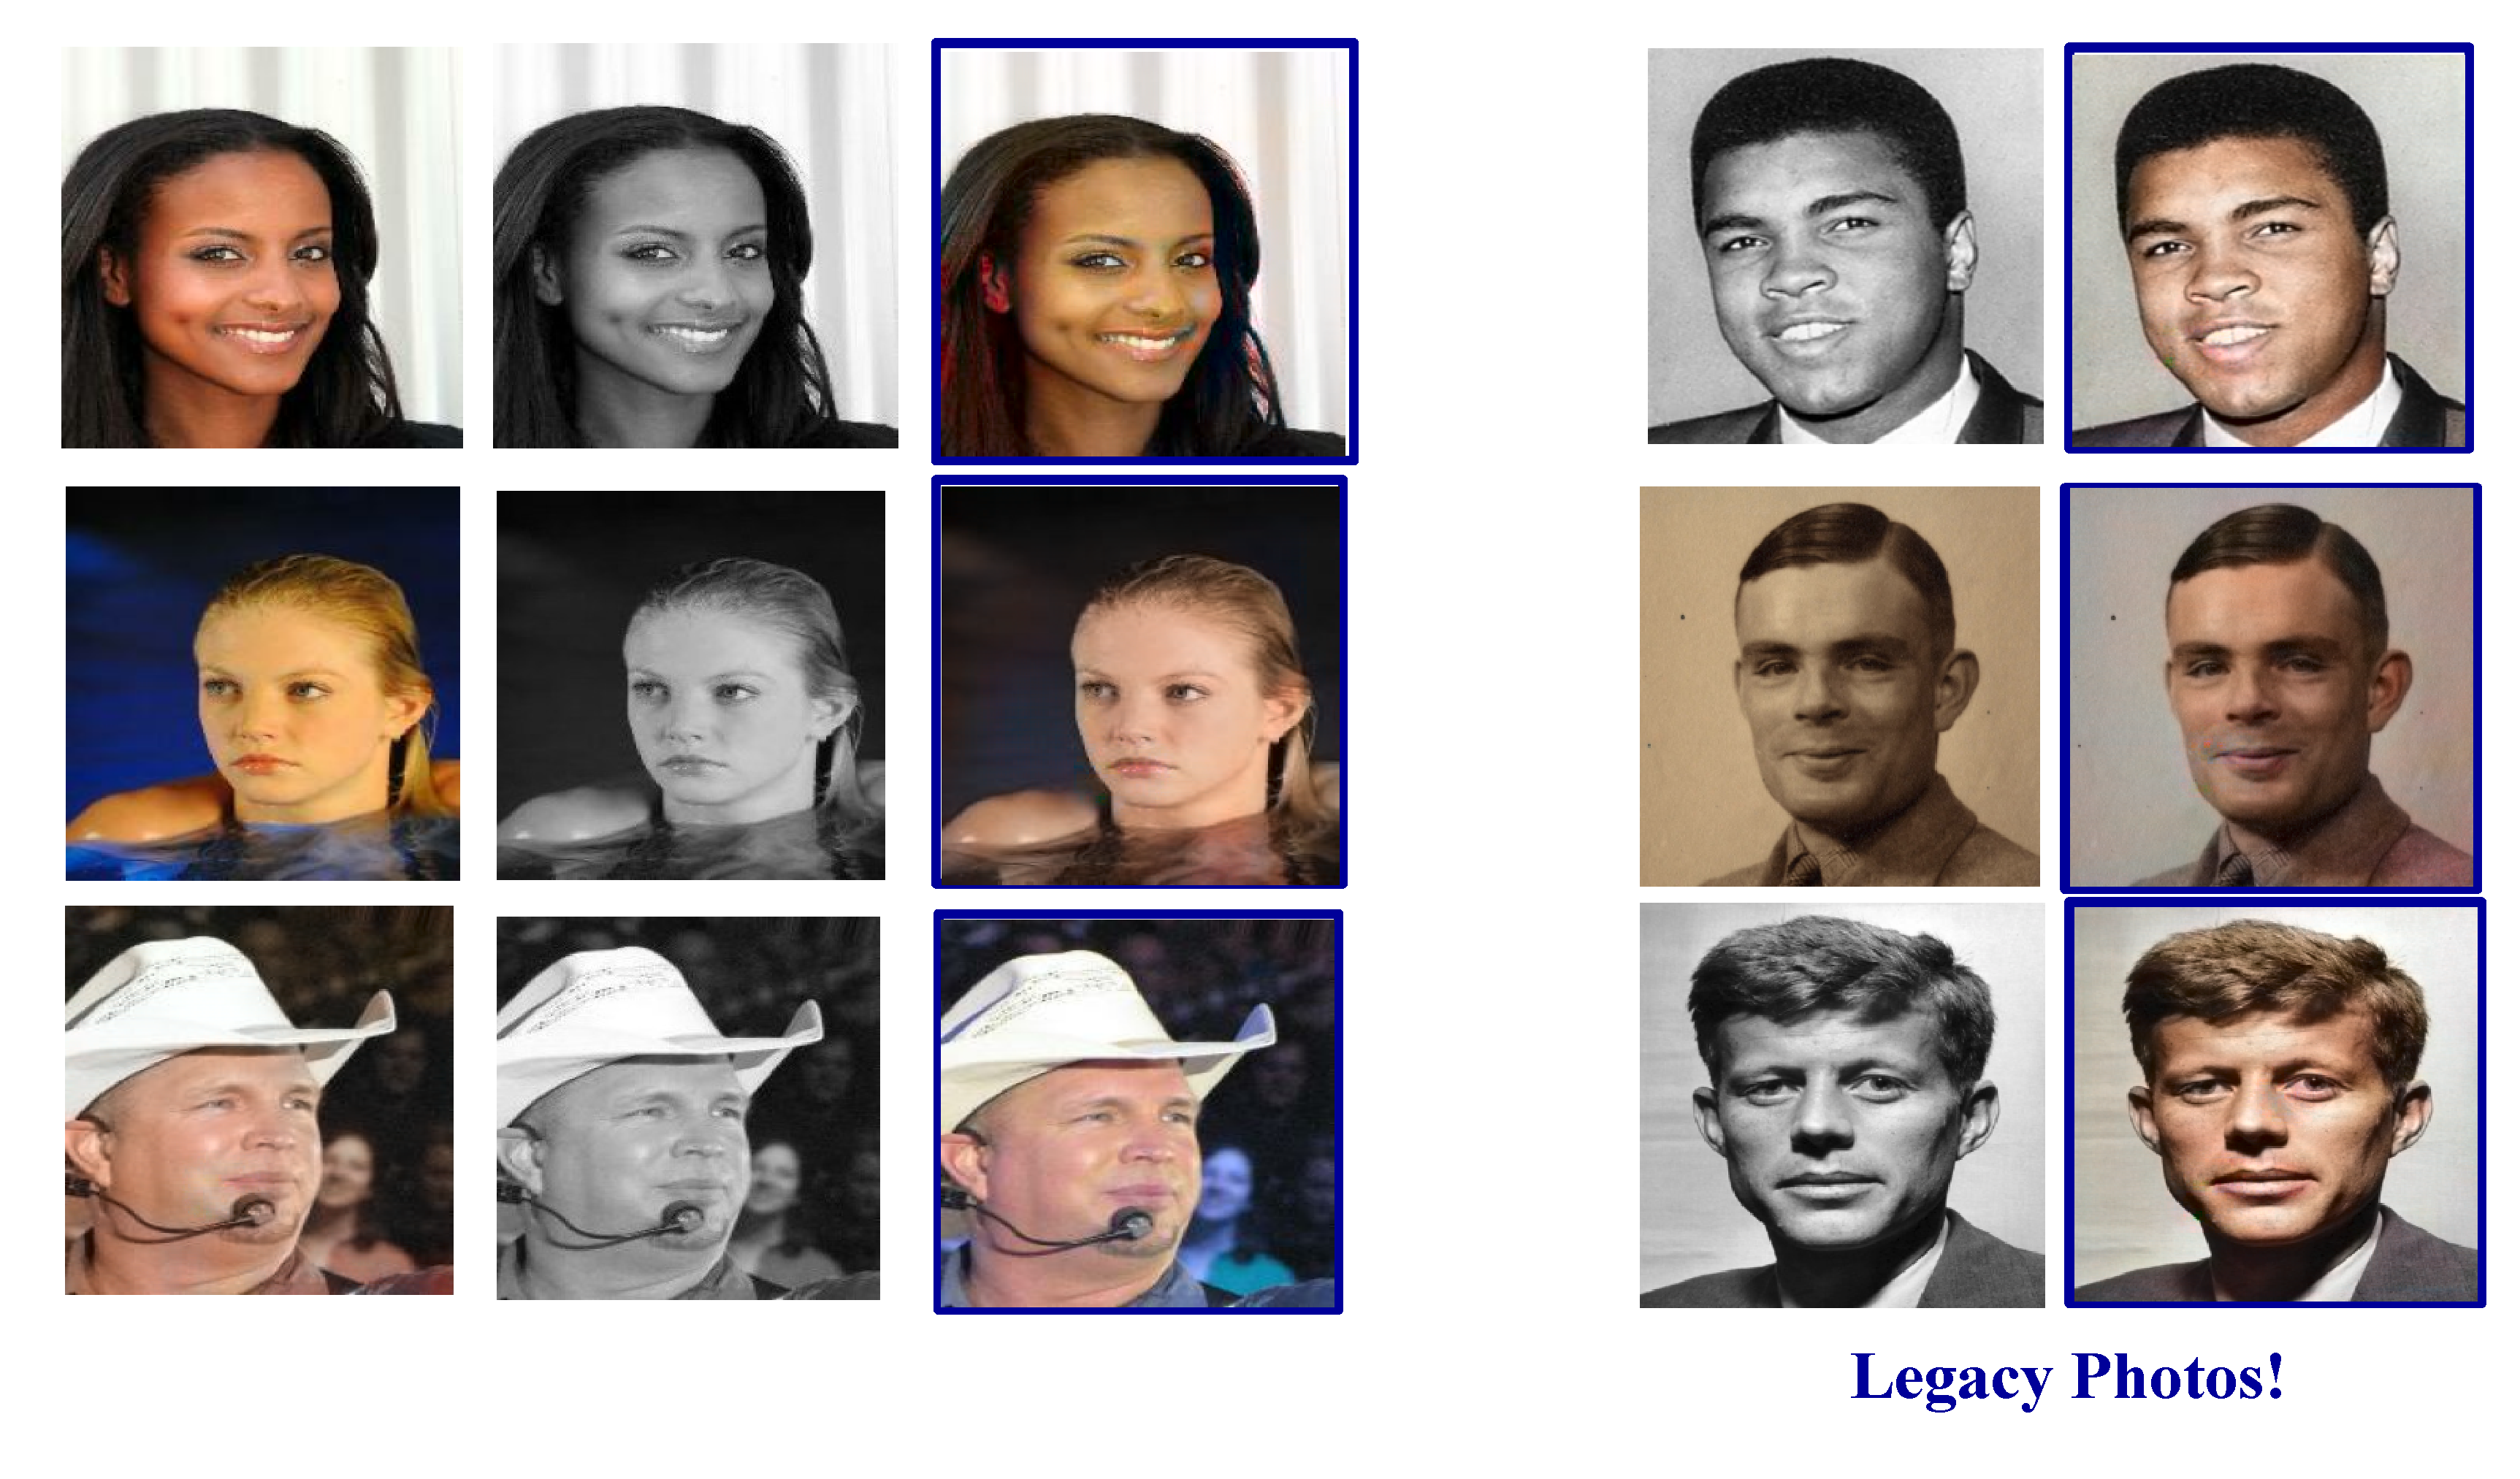
\includegraphics[width=\linewidth]{82.pdf}
\end{frame}





%%%%%%%%%%%%%%%%%%%%%%%%% GANs
\begin{frame}
\frametitle{\textbf{Generative Adversarial Networks (GANs)}}

\begin{tabular}{ll}
\begin{minipage}{0.5\textwidth}
    \begin{itemize}
        \item Two player minimax game
	     \begin{enumerate}[$-$]
           \item Discriminator \textbf{D}
           \item Generator \textbf{G}
           \end{enumerate}
       \item D is trained to discriminate between a real image and a generated image
         \end{itemize}
\end{minipage}
&
\begin{minipage}{0.5\textwidth}
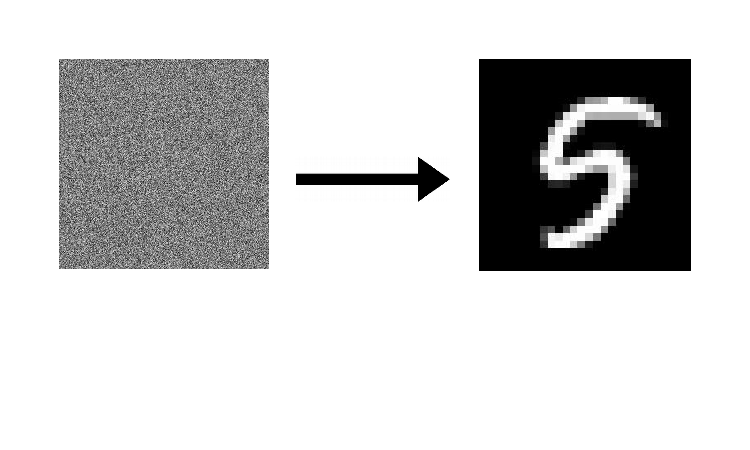
\includegraphics[width=0.9 \linewidth]{9.pdf}\end{minipage}
\end{tabular}


\begin{itemize}
\addtolength{\itemindent}{2.5mm}
  \item G is trained to generate an image that will fool D
  \item Both G and D are neural networks
      \[\min\limits_{G}\max\limits_{D} \mathbb{E}_{x \sim p_{data(x)}} [logD(\textbf{\textit{x}})] + \mathbb{E}_{z \sim p_z(z)}[log(1 - D(G(z)))]\]
  \item Conditional GANs generate images given conditional information, such as a class label.
\end{itemize}

\end{frame}
%%%%%%%%%%%%%%%%%%%%%%%


\begin{frame}
\frametitle{\textbf{GAN Variations}}
\begin{itemize}
\addtolength{\itemindent}{2.5mm}
\item Deep Convolutional GANs (DCGANs)
	   \begin{enumerate}[$-$]
         \item Bridge the gap between GANs and Deep Learning
      \end{enumerate}
\end{itemize}

\begin{tabular}{ll}
\begin{minipage}{0.57\textwidth}
   \begin{itemize}      
      \item Least Squares GANs (LSGANs)
	   \begin{enumerate}[$-$]
         \item Use a least squares loss for the discriminator
      \end{enumerate}
      \vspace{1.5mm}
      \item Energy-Based GANs (EBGANs)
	   \begin{enumerate}[$-$]
         \item Model the discriminator as an energy function
      \end{enumerate}
   \end{itemize}
\end{minipage}
&
\begin{minipage}{0.43\textwidth}
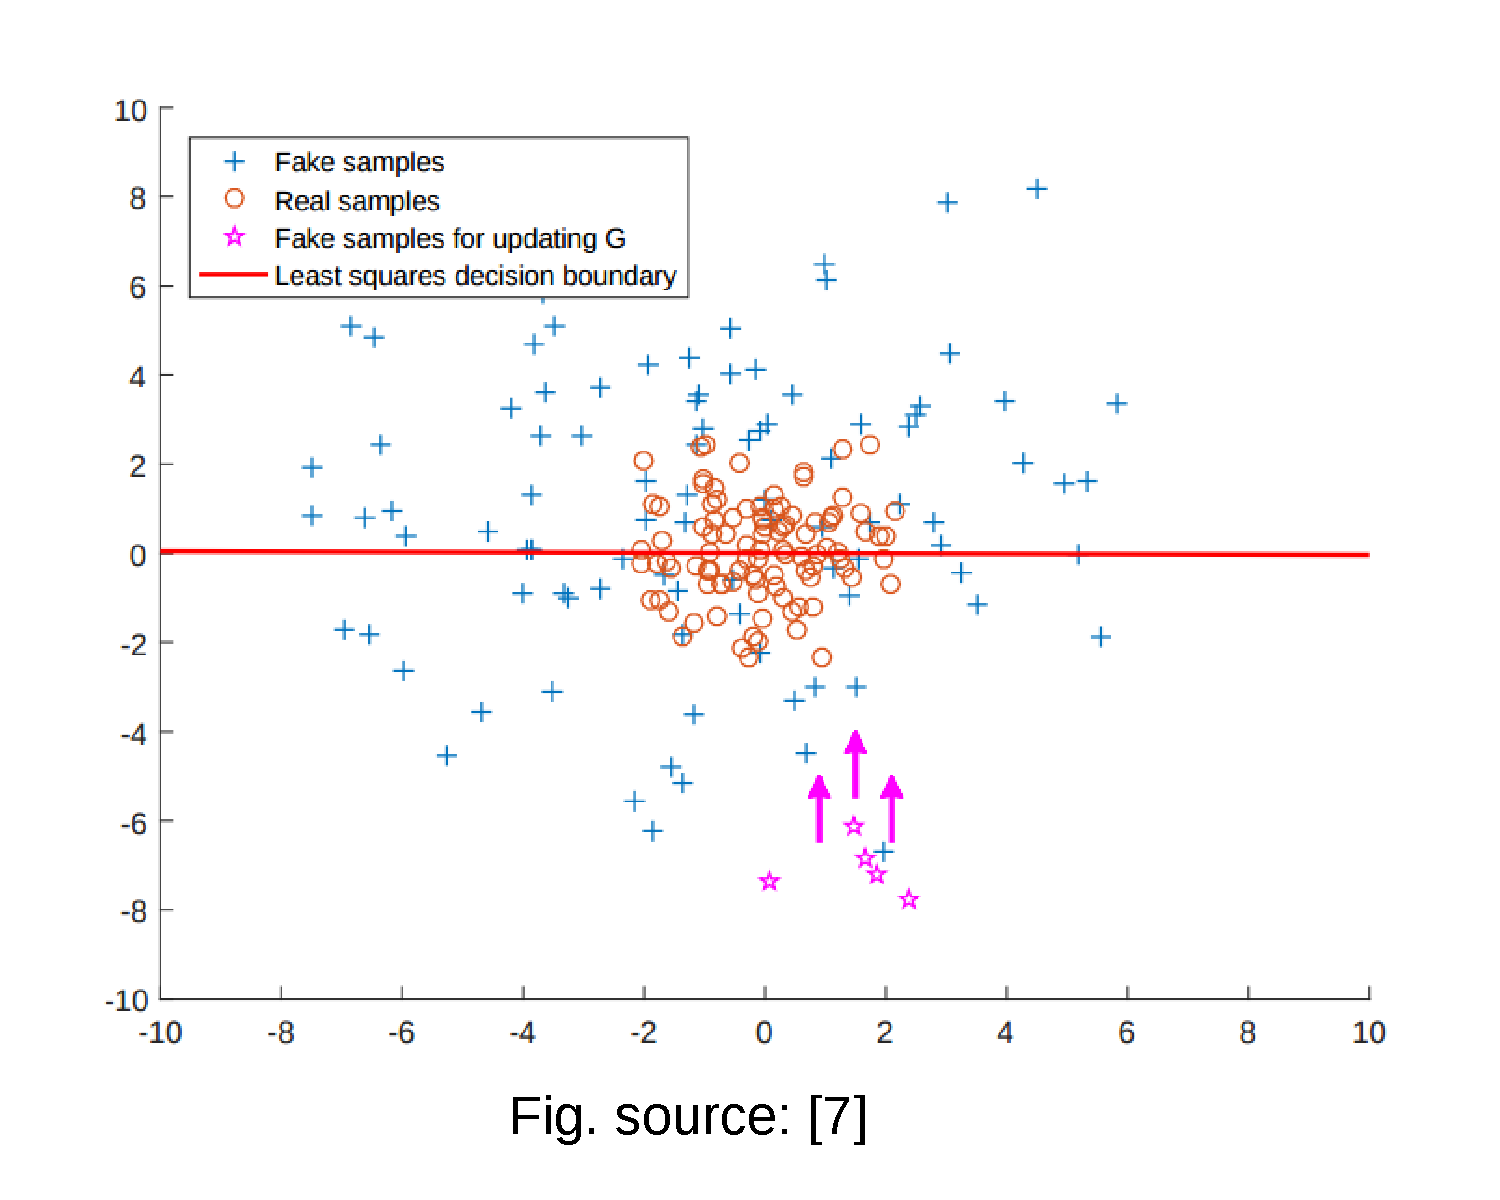
\includegraphics[width=\linewidth]{10.pdf}\end{minipage}
\end{tabular}

\begin{itemize}
\addtolength{\itemindent}{2.5mm}
  \item Wasserstein GAN (WGAN)
	   \begin{enumerate}[$-$]
         \item Minimizes the Earth Mover distance between two distributions
      \end{enumerate}
\end{itemize}


\end{frame}
%%%%%%%%%%%%%%%%%%%%%%%



\section*{Results}
\begin{frame}
\frametitle{\textbf{GAN Comparison Results}}
\centering
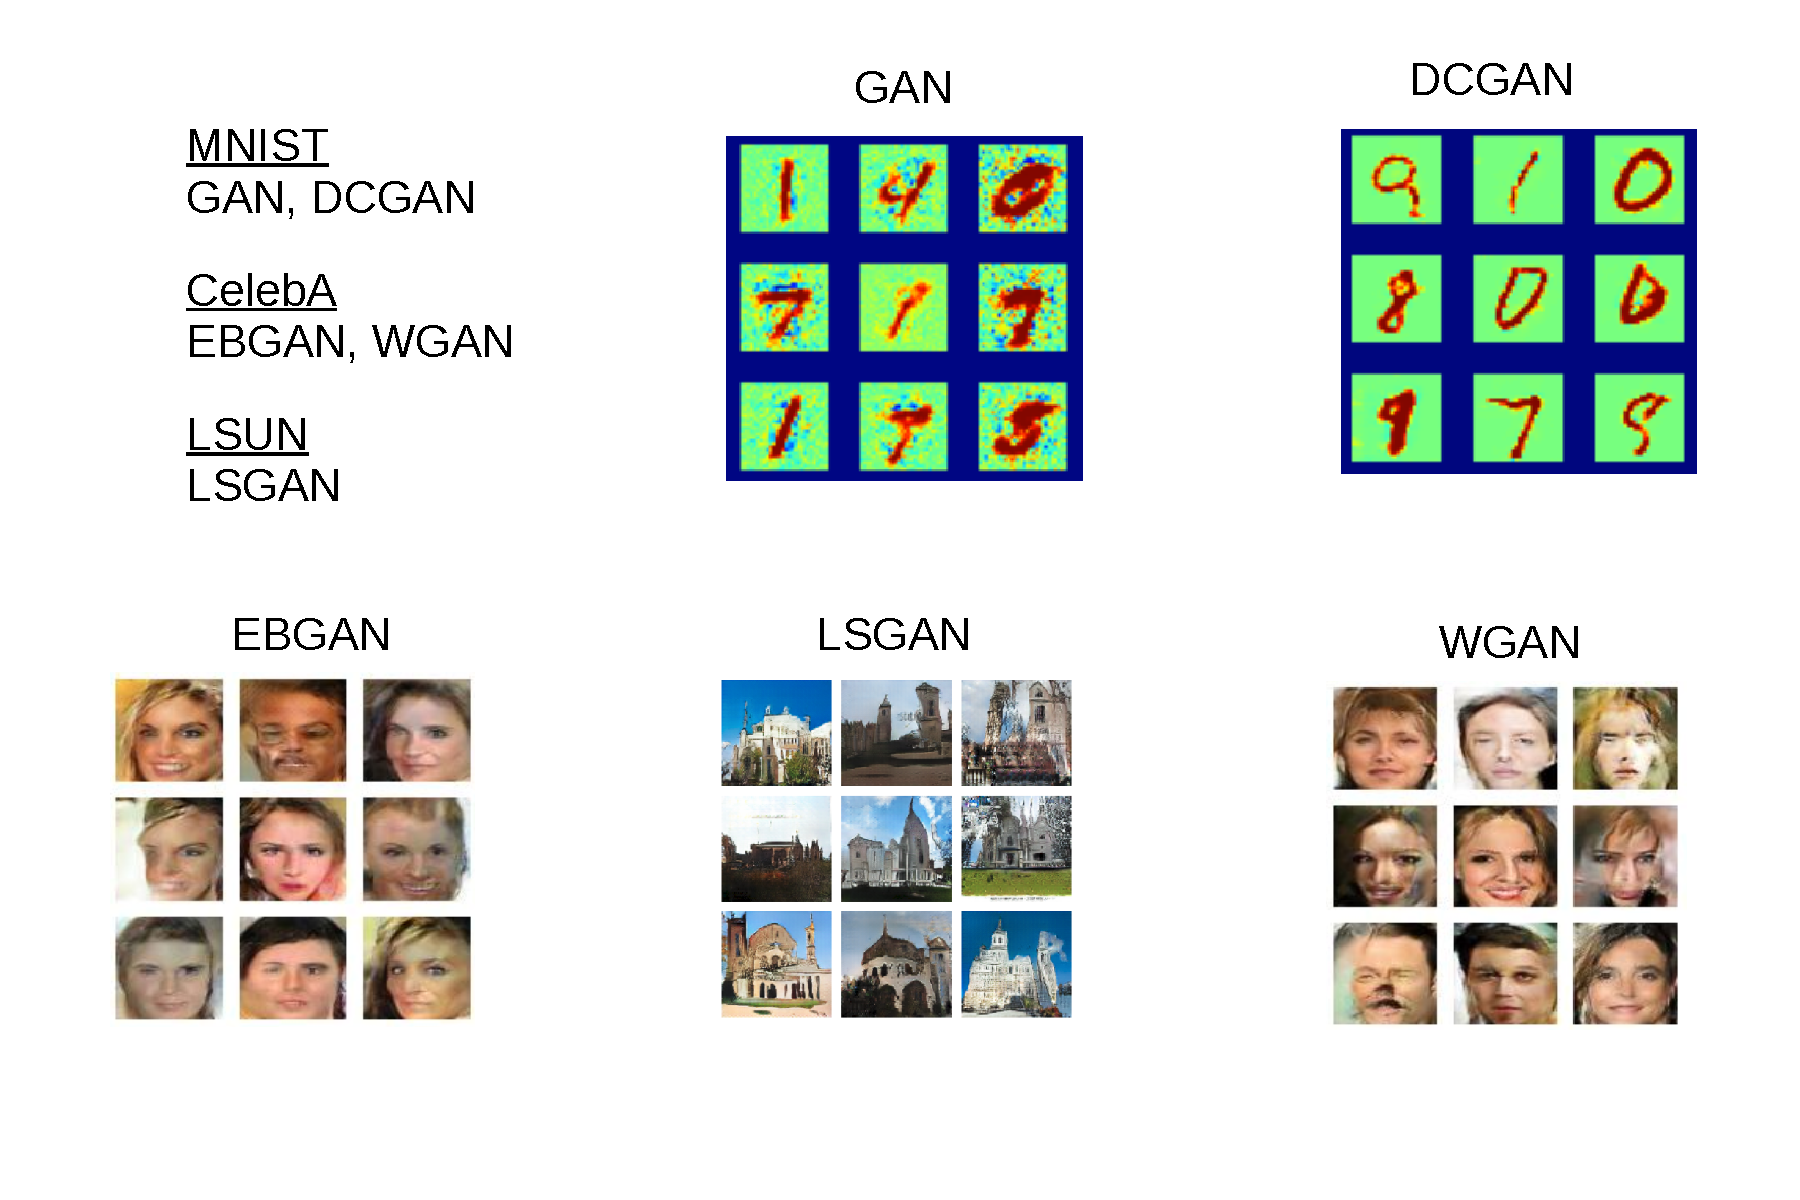
\includegraphics[width= \linewidth]{11.pdf}
\end{frame}


\begin{frame}
\frametitle{\textbf{GANs Towards Colorization}}

\begin{tabular}{ll}
\begin{minipage}{0.55\textwidth}
   \begin{itemize}      
      \item Tested two generators
	   \begin{enumerate}[$-$]
         \item Pix2Pix
         \item Colorful Image Colorization
         \vspace{1mm}
      \end{enumerate}
      \item Pix2Pix generator is  modeled as an encoder-decoder with skip connections
      \vspace{1mm}
      \item Combine L1 and L2 loss with GAN Variatons
   \end{itemize}
\end{minipage}
&
\begin{minipage}{0.5\textwidth}
\hspace{-5mm}
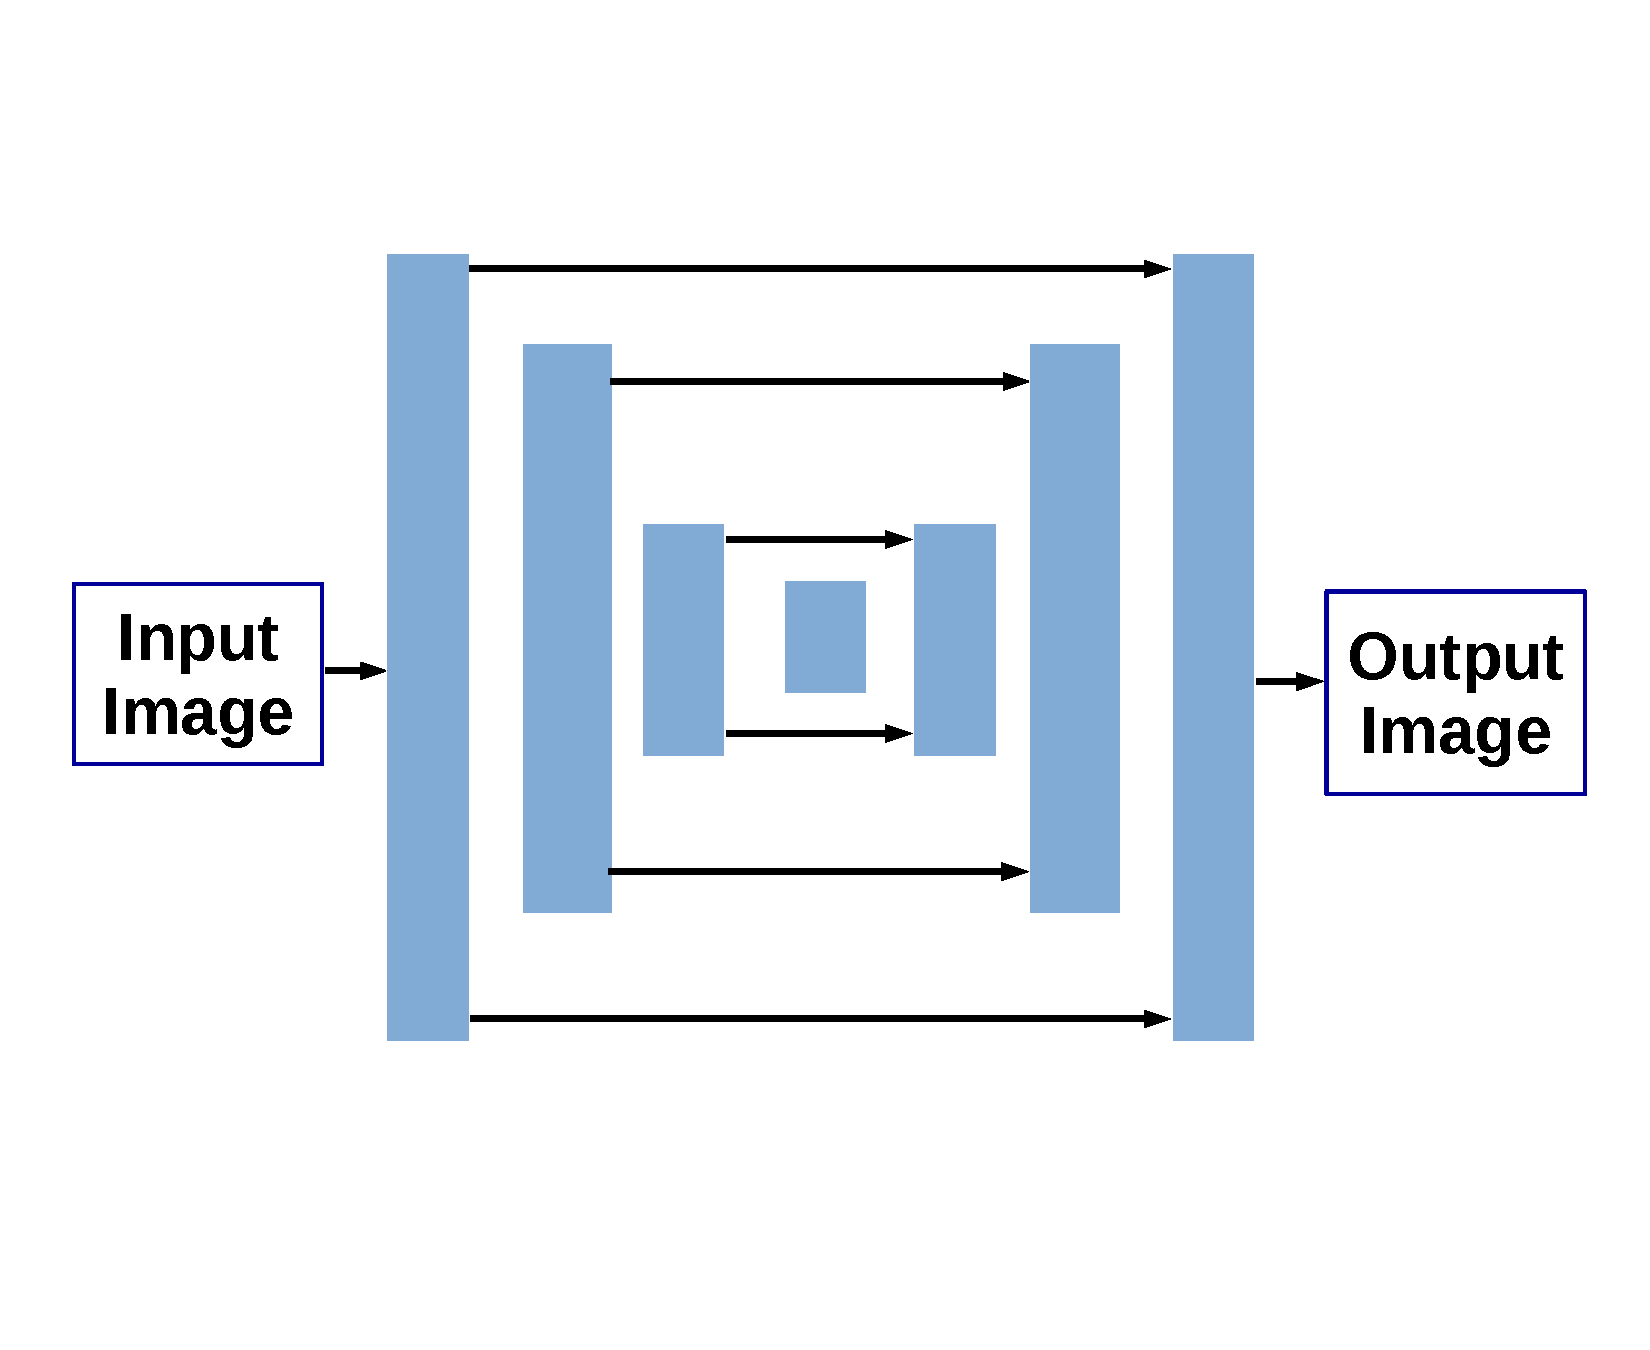
\includegraphics[width=\linewidth]{12.pdf}\end{minipage}
\end{tabular}


\end{frame}



\begin{frame}
\frametitle{\textbf{Results in Comparison}}
\centering
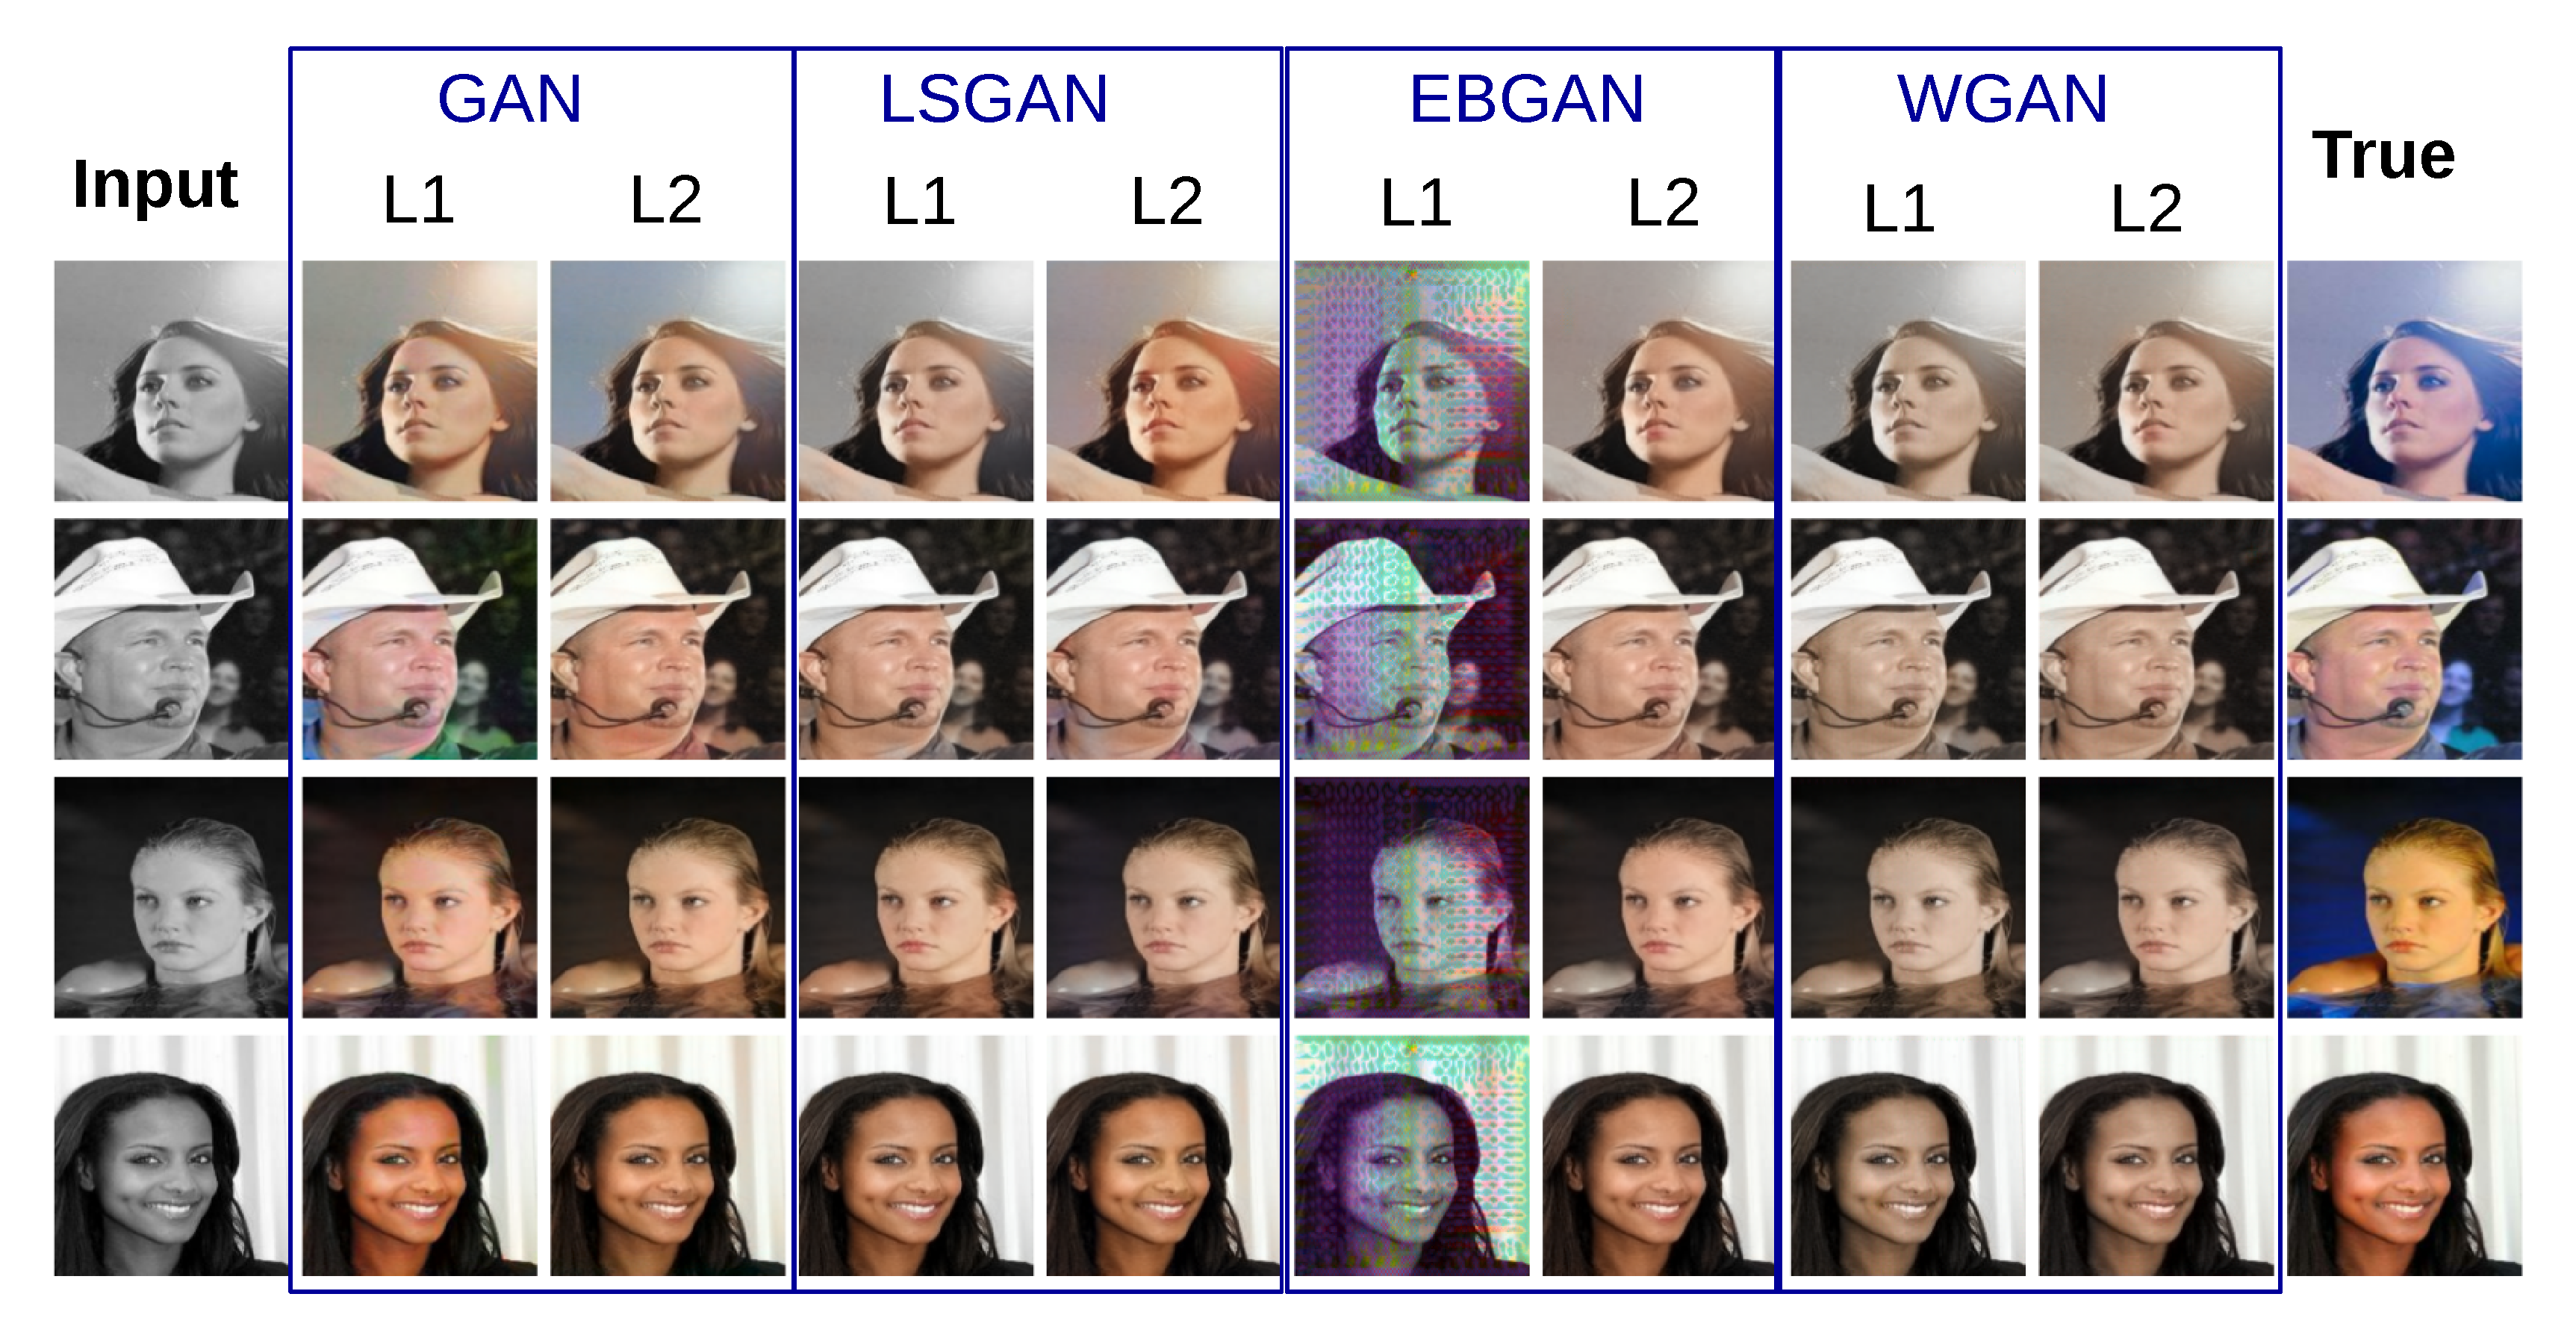
\includegraphics[width= \linewidth]{13.pdf}
\end{frame}

\begin{frame}
\frametitle{\textbf{Legacy Grayscale Results}}
\centering
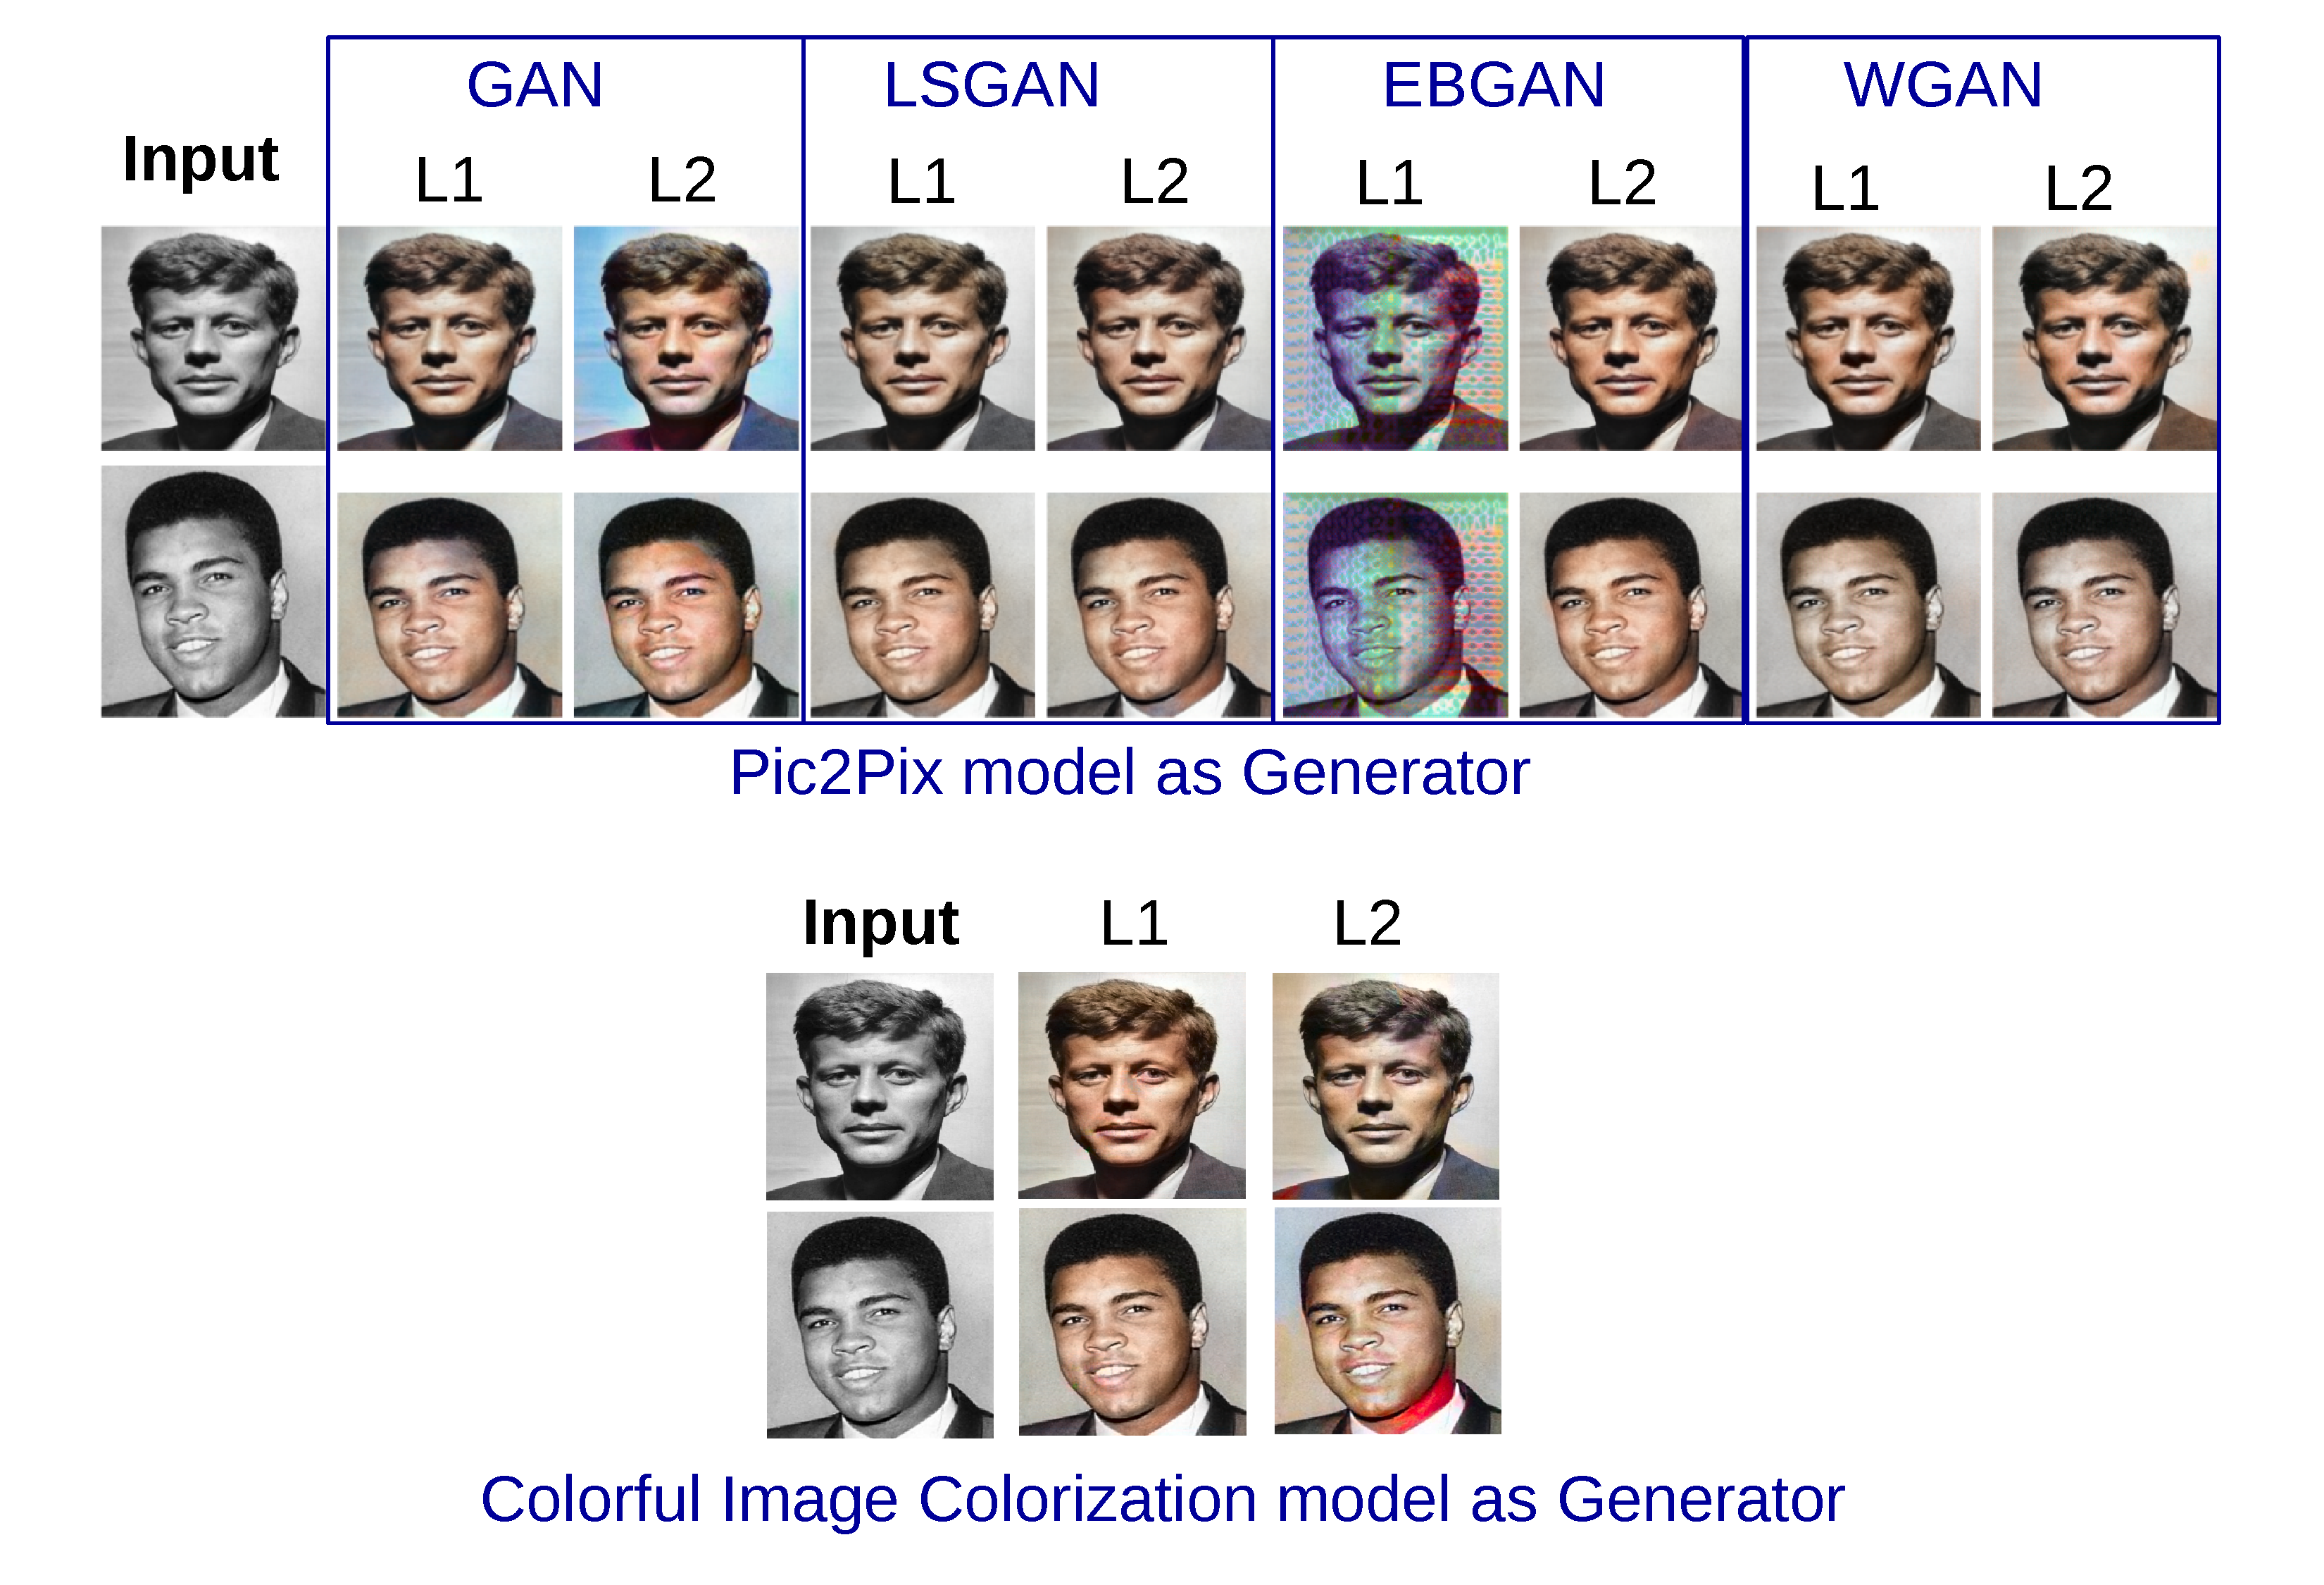
\includegraphics[width= 0.95 \linewidth]{14.pdf}
\end{frame}

\begin{frame}
\frametitle{\textbf{Lessons Learned}}

\begin{itemize}
\item Automatic colorization is difficult due to
\begin{enumerate}[$-$]
\item Ambiguity
\item Multi-modality
\end{enumerate}
\item Need large datasets to \textit{learn} colorization
\item GANs are tricky
\item Long turnover time, at least 1 to 2 days
\item End to end trainable
\item Inference is 30fps on CPU, 60fps on GPU
\end{itemize}
\end{frame}



%\begin{frame}
%\begin{quote}
%\begin{center}
%\huge{Thank you all !} \\

%\end{center}   
%\end{quote}
%\end{frame}

\begin{frame}
\frametitle{\textbf{References}}
%\footnotesize
\tiny
\begin{enumerate}
\item Richard Zhang, Phillip Isola, and Alexei A Efros. \textit{Colorful image colorization}. In European Conference on Computer Vision,
pages 649–666. Springer, 2016.
\item Huimin Lu, Yujie Li, and Seiichi Serikawa. \textit{Underwater image enhancement using guided trigonometric bilateral filter and fast
automatic color correction}. In Image Processing (ICIP), 2013 20th IEEE International Conference on, pages 3412–3416. IEEE, 2013.
\item Luz A Torres-Méndez and Gregory Dudek. \textit{Color correction of underwater images for aquatic robot inspection}. In International
Workshop on Energy Minimization Methods in Computer Vision and Pattern Recognition, pages 60–73. Springer, 2005.
\item Anat Levin, Dani Lischinski, and Yair Weiss. \textit{Colorization using optimization}. In ACM Transactions on Graphics (ToG), volume 23, pages 689–694. ACM, 2004.
\item Guillaume Charpiat, Matthias Hofmann, and Bernhard Schölkopf. \textit{Automatic image colorization via multimodal predictions}. Computer Vision–ECCV 2008, pages 126–139, 2008.
\item Goodfellow, Ian, et al. \textit{Generative adversarial nets}. Advances in neural information processing systems. 2014.
\item Mao, Xudong, et al. \textit{Least squares generative adversarial networks}. arXiv preprint ArXiv:1611.04076 (2016).
\item Arjovsky, Martin, Soumith Chintala, and Lon Bottou. \textit{Wasserstein gan}. arXiv preprint arXiv:1701.07875 (2017).
\item Zhao, Junbo, Michael Mathieu, and Yann LeCun. \textit{Energy-based generative adversarial network}. arXiv preprint arXiv:1609.03126 (2016).
\item Radford, Alec, Luke Metz, and Soumith Chintala. \textit{Unsupervised Representation Learning with Deep Convolutional Generative Adversarial Networks}. ICLR (2016): https://arxiv.org/abs/1511.06434.










\end{enumerate}
\end{frame}
\end{document}
